\section{Realisierung}

In diesem Kapitel wird die konkrete Umsetzung der Anforderungen in GWT beschrieben.
Zuerst wird die Architektur der Anwendung festgelegt. Anschließend werden konkrete
Implementierungsdetails erläutert, welche die Erstellung eigener Widgets mittels GWT und
JSNI sowie das Styling in GSS und die Lokalisierung umfassen.

\subsection{Architektur}
Um den in Kapitel \ref{sec:Anforderungen} beschriebenen Anforderungen der zwei Anwendergruppen (Gastgeber und Partygäste) gerecht zu werden, entwickeln wir zwei GWT-Anwendungen. Die Admin-Oberfläche wird als klassische Webanwendung
entwickelt, während die VoteApp für die mobile Nutzung optimiert wird. Trotzdem werden beide Anwendungen mit einer ähnlichen Softwarearchitektur implementiert (Abb. \ref{fig:Architektur-Ueberblick}).

\begin{figure}[tbh]
\centering
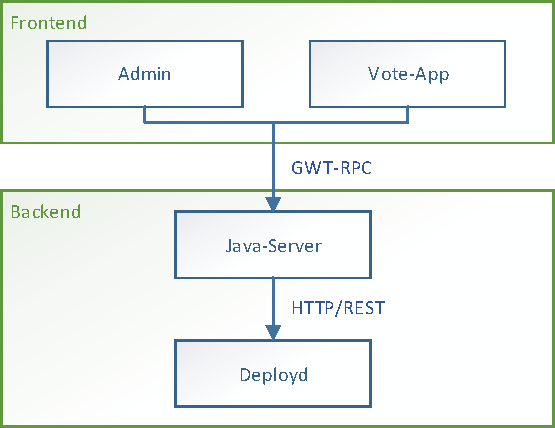
\includegraphics[width=0.7\linewidth]{Bilder/Architektur-Ueberblick}
\caption{Überblick über die Architektur der beiden Anwendungen}
\label{fig:Architektur-Ueberblick}
\end{figure}

Die Webapplikationen kommunizieren über GWT-RPC\footnote{Remote Procedure Calls werden in GWT zur Kommunikation zwischen Client und Server verwendet} mit einem Java-Server. Dieser dient als 
Proxy zum Deployd-Server und enthält selbst keine Applikationslogik. Auf diese Weise umgehen wir das Problem der Same-Origin-Policy. Der Deployed-Server ist für die Persistenz der Daten und die Anwendungslogik verantwortlich und wird über eine REST-Schnittstelle angesprochen (s. Anhang \ref{anh:rest}).

\subsubsection{Frontend}
Innerhalb der Frontend-Anwendungen wird MVP zur Trennung von Steuerung und Anzeige der Oberfläche implementiert. Der Zugriff auf das Model wird über GWT-RPC-Services ermöglicht, die Anfragen an den Java-Server im Backend durchführen (Abb. \ref{fig:MVP-mit-Service}).

\begin{figure}[tbh]
\centering
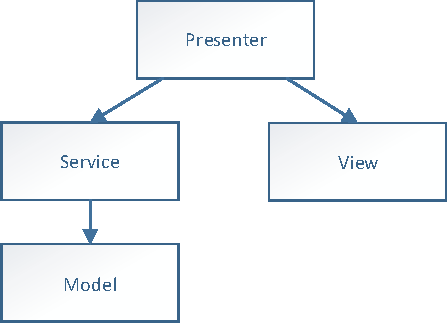
\includegraphics[width=0.6\linewidth]{Bilder/MVP-mit-Service}
\caption{MVP mit Service}
\label{fig:MVP-mit-Service}
\end{figure}

In der nachfolgenden Übersicht werden die erstellten View-Presenter-Paare des Admins vorgestellt:
\begin{description}
	\item[PartyManagamentView und -Presenter:] Verwalten einer Party im Admin
	\item[SongManagementView und -Presenter:] Verwalten der Songsammlung im Admin
	\item[LanguageSelectionView und -Presenter:] Ändern der Anzeigesprache im Admin
\end{description}

Im Gegensatz zum Admin besteht die VoteApp lediglich aus einem View-Presenter-Paar:

\begin{description}
	\item[VoteAppView und -Presenter:] Teilnahme an einer Party als Gast über die VoteApp
\end{description}

\subsubsection{Backend}
Wie zuvor beschrieben, besteht das Backend aus einem Java-Server und Deployd.
Zur Einrichtung von Deployd sind zwei Schritte
notwendig:
\begin{itemize}
	\item Definition der verwendeten Ressourcen
	\item Hinterlegung von eigenem JavaScript-Code\footnote{Der Code wird in JavaScript hinterlegt, da Deployd auf node.js basiert.}, der beim Zugriff auf die Ressourcen ausgeführt wird
\end{itemize}
Auf diese Weise konnten wir das notwendige Datenmodell und die
dazugehörige Anwendungslogik hinterlegen.

Die von uns definierten Ressourcen umfassen:
\begin{description}
	\item[/party] Daten der aktuellen Party
	\item[/playlist] Die aktuelle Playlist (Songs und deren Votes)
	\item[/currentsong] Der Song, der gerade gespielt wird
	\item[/song] Songsammlung, aus der Songs für die Playlist gewählt werden
\end{description}

\subsection{Eigene Widgets}
Im Rahmen der Realisierung sind viele eigene Widgets entstanden. Um ein eigenes Widget zu implementieren, leitet man von der Klasse Composite ab und ruft im Konstruktor die Methode initWidget auf. Neben kleineren Hilfskomponenten haben wir vor allem die Views als eigene Widgets realisiert.

Im Folgenden werden exemplarisch die Hilfskomponenten InputBox und PlayListEntryWidget sowie die SongListView vorgestellt.

\subsubsection{PlayListEntryWidget}
Das PlayListEntryWidget ist ein touch-freundliches Widget für die VoteApp. Es dient der Darstellung eines Eintrags in der Playlist mit zusätzlicher Möglichkeit zum Voten. Es besteht aus zwei Labels zum Anzeigen des Titels und des Interpreten und zwei Buttons zum Voten. 

\begin{figure}[tbh]
	\centering
	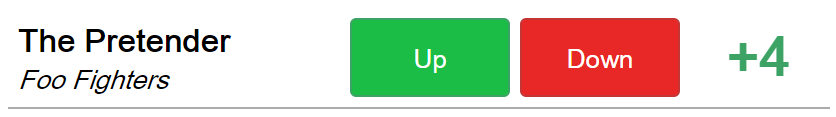
\includegraphics[width=0.7\linewidth]{Bilder/PlayListEntry}
	\caption{Eintrag in der Playlist mit Vote-Möglichkeiten}
	\label{fig:PlayListEntry}
\end{figure}

Abbildung \ref{fig:PlayListEntryClass} zeigt die Schnittstellenbeschreibung des PlayListEntryWidget. Im Konstruktor werden die Labels Interpret und Titel mit den Daten aus dem PlayListEntry initialisiert. Des Weiteren werden Click-Handler für die beiden Buttons hinzugefügt, welche die onUpVote- bzw. onDownVote-Methoden des Interfaces VoteListener aufrufen. Über die setVoteListener-Methode kann ein Listener für die Vote-Eingaben registriert werden.

\begin{figure}[tbh]
	\centering
	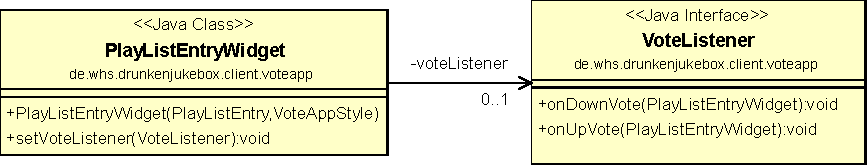
\includegraphics[width=1.0\linewidth]{Bilder/PlayListEntry.pdf}
	\caption{Schnittstellenbeschreibung des PlayListEntryWidget}
	\label{fig:PlayListEntryClass}
\end{figure}


\subsubsection{InputBox}
Die InputBox ist eine simple Hilfskomponente, die eine TextBox mit einem Label kombiniert:

\begin{figure}[H]
\centering
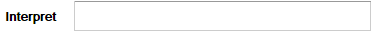
\includegraphics[width=0.7\linewidth]{Bilder/InputBox}
\caption{InputBox für den Interpreten eines Songs}
\label{fig:InputBox}
\end{figure}

Abbildung \ref{fig:InputBoxClass} zeigt die Schnittstellenbeschreibung der InputBox. Im Konstruktor wird neben dem Label-Text auch der CSS-Style übergeben, um flexibel den Style verschiedener Instanzen mittels Dependency Injection anpassen zu können. Über die Methode setFocus kann der Fokus auf die TextBox gesetzt werden. Die Methoden setText, getText und clear sind zur Manipulation der Eingabe vorgesehen.

\begin{figure}[H]
\centering
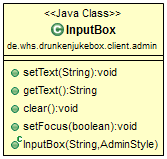
\includegraphics[width=0.3\linewidth]{Bilder/InputBoxClass}
\caption{Schnittstellenbeschreibung der InputBox}
\label{fig:InputBoxClass}
\end{figure}


\newpage
\subsubsection{SongListView}
Die SongListView besteht aus einer TextBox für die Suche, einer ListBox und einem Button zur Erstellung eines neuen Songs:

\begin{figure}[H]
\centering
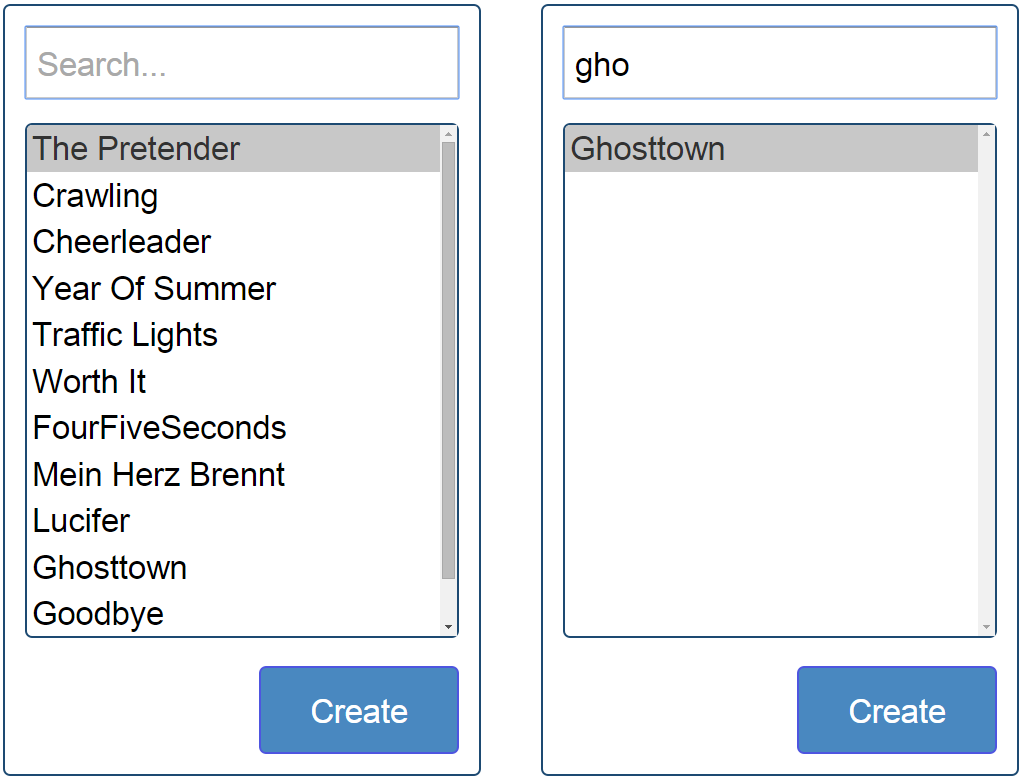
\includegraphics[width=0.65\linewidth]{Bilder/SongListView}
\caption{Liste mit Suchmöglichkeit zur Verwaltung der Songs}
\label{fig:SongListView}
\end{figure}

Grundsätzlich haben wir alle Views in Form von Interfaces deklariert. Abbildung \ref{fig:SongListViewClass} zeigt das Interface für die SongListView, dass alle benötigten Funktionen zum Umgang mit dem Widget bereitstellt. Beispielsweise können über die Methode getSongsListBox Change-Handler registriert werden. Diese werden aufgerufen, sobald sich die Selektion der ListBox ändert. Über die Methode getSelectedIndex kann daraufhin der Index des ausgewählten Songs abgefragt werden, um diesen in einer anderen View anzuzeigen.

\begin{figure}[H]
\centering
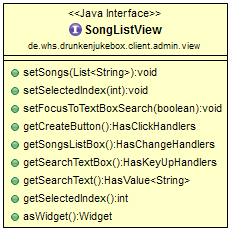
\includegraphics[width=0.4\linewidth]{Bilder/SongListViewClass}
\caption{Schnittstellenbeschreibung der SongListView}
\label{fig:SongListViewClass}
\end{figure}


\subsection{Styles in GSS}
Für das Styling der beiden GWT-Anwendungen verwenden wir GSS\footnote{\url{https://code.google.com/p/closure-stylesheets/}}. Da es unterschiedliche Anforderungen
an Deskop- und Mobilanwendungen gibt, werden zwei Stylesheet-Dateien verwendet.

Um die Styles im Java-Code verwenden zu können, müssen diese mit dem AppResources-Interface\footnote{Dieses Interface erbt von dem GWT-Interface ClientBundle} verbunden werden.
In diesem Projekt legen wir alle Ressourcen, zu denen auch Stylesheets zählen, in
einem separaten Package (de.whs.drunkenjukebox.resources) ab. Wie Abbildung
\ref{fig:GSS} zeigt, können so beide Anwendungen AppResources verwenden
und nur den jeweils benötigten Style nachladen.

\begin{figure}[tbh]
\centering
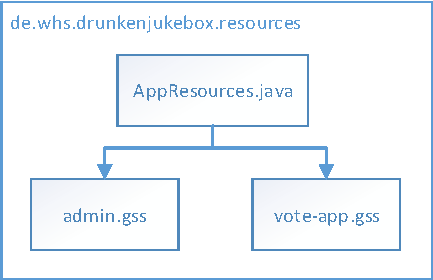
\includegraphics[width=0.5\linewidth]{Bilder/GSS}
\caption{Verknüpfung der GSS-Dateien mit Java}
\label{fig:GSS}
\end{figure}


\subsection{Lokalisierung}
Beide Anwendungen sollen lokalisiert in Deutsch und Englisch angeboten werden.
Im Admin soll es möglich sein, die Sprache über die Oberfläche zu ändern, während
in der VoteApp die Sprache automatisch ausgewählt werden soll.

\subsubsection{Properties-Dateien}

Zur Lokalisierung werden Properties-Dateien\footnote{\url{http://www.gwtproject.org/doc/latest/DevGuideI18n.html}} verwendet, welche über Interfaces
mit dem Java-Code verknüpft werden. Es gibt zwei Arten von übersetzbaren Texten:
\begin{description}
	\item[Statisch:] Text ohne Platzhalter
	\item[Dynamisch:] Text mit einem oder mehreren Platzhaltern
\end{description}
Diese Arten werden in GWT unterschiedlich behandelt. Für statische Texte muss
von Constants und für dynamische Texte von Messages abgeleitet werden. In den Interfaces können Fallback-Texte hinterlegt werden, die angezeigt werden, wenn keine passende Übersetzung in den Properties-Dateien gefunden wurde. Als
Fallback-Sprache verwenden wir Englisch, sodass wir nur Properties-Dateien für
die deutsche Übersetzung anlegen müssen.

\begin{figure}[tbh]
\centering
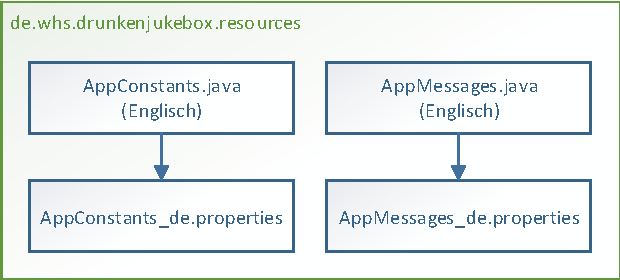
\includegraphics[width=0.7\linewidth]{Bilder/Lokalisierung}
\caption{Übersetzung mittels Properties-Dateien}
\label{fig:Lokalisierung}
\end{figure}

Abbildung \ref{fig:Lokalisierung} zeigt, dass die Übersetzungsdateien in dem
de.whs.drunkenjukebox.resources-Package abgelegt sind. Um weitere
Übersetzungen hinzuzufügen, müssen hier lediglich neue Properties-Dateien mit
dem entsprechenden Sprachkürzel angelegt und gefüllt werden.


\subsubsection{Wahl der Sprache}
In GWT kann die anzuzeigende Sprache über einen URL-Parameter bestimmt werden. Für die Admin-Oberfläche rufen wir die eigene URL
mit dem Parameter locale auf, um die vom Anwender
gewünscht Sprache anzuzeigen. Die zur Auswahl stehenden Sprachen werden dem Benutzer als Bilder angezeigt, auf denen Click-Handler den notwendigen Wechsel der URL herbeiführen.
\begin{lstlisting}[language=Java]
@Override
public void onClick(ClickEvent event) {
	String newUrl = Window.Location.getPath() + "?locale=de";
	Window.Location.assign(newUrl);
}
\end{lstlisting}
In der VoteApp soll die im Browser eingestellte Sprache verwendet werden. Dazu reicht ein Eintrag in dem GWT-Modul
der Anwendung:
\begin{lstlisting}[language=XML]
<set-configuration-property name="locale.useragent" value="Y"/>
\end{lstlisting}

\subsection{JSNI}
Die Eingabe des eigenen Drunken-Index soll mithilfe eines Schiebereglers erfolgen. GWT enthält jedoch kein entsprechendes  Benutzerelement, weswegen wir uns überlegt haben mithilfe von jQuery-UI\footnote{https://jqueryui.com/} und JSNI einen HTML5-Slider zu implementieren. Dessen Verwendung sollte wie ein natives GWT-Widget wirken. Dazu war es nötig die JSNI-Funktionen vor der direkten Benutzung in ein Custom-Widget zu kapseln. 

JSNI ermöglicht es in einer GWT-Applikation natives JavaScript zu schreiben, welches bei der Kompilierung der Anwendung übernommen wird. Dies ermöglicht die direkte Integration von JavaScript in Java-Code.

Wir haben ein neues Widget erstellt, das Methoden zum Setzen und Lesen des Slider-Wertes ermöglicht. Weiter wurde ein Slider-Listener implementiert, welcher beim "'onSlide"'-Event aufgerufen wird und den aktuellen Wert übergibt. Das Custom-Widget erstellt ein neues "`div"'-Element, in welchem mithilfe von jQuery-UI ein Slider-Element eingebettet wird. Aus dem Javascript heraus wird die "'onSlide"'-Methode der kapselnden Java-Klasse aufgerufen. Zur Benutzung des Sliders müssen die entsprechenden jQuery und jQuery-UI Bibliotheken im Head der HTML-Datei eingebunden werden. Abbildung \ref{fig:DISlider} zeigt den fertigen Slider.

\begin{figure}[tbh]
\centering
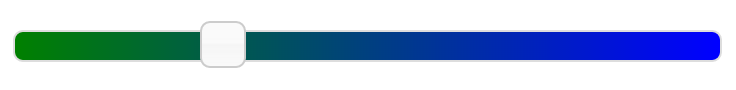
\includegraphics[width=0.7\linewidth]{Bilder/DISlider}
\caption{JavaScript-Slider über JSNI}
\label{fig:DISlider}
\end{figure}

